\documentclass[conference]{IEEEtran}

\IEEEoverridecommandlockouts
\usepackage{cite}
\usepackage{amsmath,amssymb,amsfonts}
\usepackage{graphicx}
\usepackage{textcomp}
\usepackage{xcolor}
\usepackage{booktabs}
\usepackage{hyperref}
\usepackage{multirow}
\usepackage{algorithm}
\usepackage{algorithmic}
\usepackage{subcaption}
\usepackage{tikz}
\usetikzlibrary{shapes,arrows,positioning,fit,calc}

\def\BibTeX{{\rm B\kern-.05em{\sc i\kern-.025em b}\kern-.08em
    T\kern-.1667em\lower.7ex\hbox{E}\kern-.125emX}}

\title{AgriDSS: An Implemented AI-Based Integrated Agricultural\\
Decision Support System with Multimodal Interaction\\
and Multilingual Mobile Interface}

\author{
\IEEEauthorblockN{Harish Saini\IEEEauthorrefmark{1}, Navya Bhumbak\IEEEauthorrefmark{1}, Bhavya Mittal\IEEEauthorrefmark{1}, Anisha Gupta\IEEEauthorrefmark{1}}
\IEEEauthorblockA{\IEEEauthorrefmark{1}University of Petroleum and Energy Studies (UPES), Dehradun, India\\
Email: \{harish.126796, Navya.120383, Bhavya.119005, anisha.28331\}@stu.upes.ac.in}
}

\begin{document}

\maketitle

\begin{abstract}
Smallholder farmers in developing nations face compounded challenges including limited access to agronomic expertise, unpredictable weather, and fragmented decision-support tools. Existing AI-based agricultural solutions typically address isolated tasks - crop recommendation, disease detection, or yield forecasting - without integration, multilingual support, or offline capability, limiting their practical utility. This paper presents AgriDSS, a \textbf{fully implemented} integrated agricultural decision support system that unifies five tightly coupled analytical modules - crop recommendation, plant disease detection, yield forecasting, ET\textsubscript{0}-based irrigation advisory, and AI-powered action planning - within a single multilingual mobile platform. We formalize the system's multi-stage pipeline as the \textbf{HARVEST} (Hybrid Agri-intelligence with Real-time Verification, ET\textsubscript{0} Scheduling, and Transformer-based diagnostics) framework, a novel orchestration pattern combining statistical ML inference with LLM-based contextual reasoning and a three-tier graceful degradation cascade. The backend, built on FastAPI, orchestrates a Vision Transformer (ViT) for 38-class leaf disease classification, a Random Forest classifier (99.3\% test accuracy, 22 crop classes) for soil--weather-aware crop recommendation, a Random Forest Regressor trained on a 15-dimensional feature vector with log1p target transformation ($R^2 = 0.94$) for yield prediction, and a Hargreaves--Samani evapotranspiration model for irrigation scheduling. A Groq-hosted LLaMA 3.3 70B model serves as a context-aware reasoning engine across all modules. The React Native (Expo) mobile application supports full interface localization in English, Hindi, and Punjabi, with a voice-operated interface using Whisper-Large-V3 for multilingual speech recognition and intent classification. SHAP-based model interpretability analysis reveals that crop type dominates yield predictions (mean $|\text{SHAP}| = 1.46$), followed by geographic coordinates and soil pH. An offline-first architecture with on-device knowledge base, TTL-based caching, and automatic queue synchronization ensures functionality without network connectivity. Empirical evaluation across four candidate regressors demonstrates sub-2-second disease inference latency and 26--38\% water savings through ET\textsubscript{0}-optimized irrigation scheduling compared to traditional flood irrigation practices.
\end{abstract}

\begin{IEEEkeywords}
Precision Agriculture, Decision Support System, Crop Recommendation, Plant Disease Detection, Vision Transformer, Yield Forecasting, SHAP Explainability, Multilingual Interface, Offline-First Architecture, Evapotranspiration, Hybrid ML-LLM Framework
\end{IEEEkeywords}

\section{Introduction}

Agriculture sustains the livelihoods of over 58\% of India's population, yet the majority of smallholder farmers - operating plots under 2 hectares - continue to rely on generational heuristics for critical decisions regarding crop selection, pest management, irrigation scheduling, and market timing~\cite{b1}. The consequences of suboptimal agronomic decisions are severe: India loses an estimated 15--25\% of potential crop yield annually to preventable disease, inefficient water use, and mismatched crop--soil combinations~\cite{b2,b3}.

Recent advances in machine learning (ML), computer vision, and large language models (LLMs) have produced promising standalone agricultural tools---deep learning classifiers for leaf disease~\cite{b12,b13}, Random Forest models for crop recommendation~\cite{b8}, and gradient-boosted regressors for yield prediction~\cite{b6}. However, these contributions overwhelmingly exist as isolated research prototypes evaluated on benchmark datasets, with minimal attention to deployment, integration, or end-user accessibility~\cite{b5}. A farmer simultaneously needs to know \textit{which crop to plant} given current soil conditions, \textit{whether a leaf anomaly is treatable}, \textit{what yield to expect} given weather forecasts, \textit{how much water to apply} today, and \textit{what tasks to prioritize} this week. Addressing these needs through disconnected tools places an unreasonable cognitive burden on users with limited digital literacy.

Three critical gaps persist in the literature:

\begin{enumerate}
    \item \textbf{Integration gap:} No existing deployed system unifies crop recommendation, disease detection, yield prediction, irrigation advisory, and action planning under a shared data pipeline consuming common soil, weather, and location context.
    \item \textbf{Accessibility gap:} Most agricultural AI tools operate exclusively in English and require stable internet connectivity---assumptions that fail for 70\% of Indian farmers who speak regional languages and operate in low-connectivity rural areas~\cite{b4}.
    \item \textbf{Explainability gap:} ML-based recommendations are typically presented as opaque outputs without contextual reasoning, reducing farmer trust and adoption~\cite{b14}.
\end{enumerate}

This paper addresses all three gaps by presenting \textbf{AgriDSS}, a fully implemented, field-tested agricultural decision support system. Unlike prior work that proposes architectures or evaluates models in isolation, AgriDSS is an operational end-to-end platform currently deployed on Android devices. The contributions of this paper are:

\begin{itemize}
    \item The \textbf{HARVEST framework} (Hybrid Agri-intelligence with Real-time Verification, ET\textsubscript{0} Scheduling, and Transformer-based diagnostics) - a formalized multi-stage orchestration pipeline that combines statistical ML inference with LLM-based contextual reasoning through a novel three-tier graceful degradation cascade (ML+LLM $\rightarrow$ ML-only $\rightarrow$ static fallback), ensuring system availability across all connectivity conditions.
    \item A \textbf{fully implemented} multi-module backend integrating five analytical services---crop recommendation (Random Forest, 99.3\% accuracy, 22 classes), plant disease detection (ViT, 38 classes), yield forecasting (Random Forest Regressor, 15 features, $R^2 = 0.94$), ET\textsubscript{0}-based irrigation scheduling (Hargreaves--Samani~\cite{b22} with FAO-56 $K_c$~\cite{b23}), and LLM-powered action planning---consuming shared weather, soil, and geolocation context through a unified FastAPI data pipeline.
    \item \textbf{Rigorous model selection and interpretability:} Comparative evaluation of four regression architectures (Decision Tree, Random Forest, XGBoost~\cite{b25}, LightGBM~\cite{b26}) with SHAP-based~\cite{b21} feature attribution analysis revealing crop type as the dominant predictor (mean $|\text{SHAP}| = 1.46$), providing agronomically interpretable model behavior.
    \item A \textbf{multilingual mobile application} with complete interface localization in English, Hindi, and Punjabi, and a \textbf{multimodal interaction system} combining touch, voice (Whisper-Large-V3 ASR with LLM-based intent classification routing to 10 screen targets), and text-to-speech for hands-free field operation.
    \item An \textbf{offline-first architecture} with TTL-based caching, an on-device trilingual knowledge base (15 topic areas), an automatic offline queue with reconnection synchronization, and graceful degradation across all modules.
    \item An \textbf{explainability framework} providing confidence badges, data source attribution tags, expandable reasoning cards, and weather-aware safety alerts---implemented as reusable UI components across all advisory screens.
    \item Quantitative evaluation demonstrating sub-2-second disease inference, 99.3\% crop recommendation accuracy, and 26--38\% irrigation water savings against traditional methods.
\end{itemize}

The remainder of this paper is organized as follows. Section~II reviews related work. Section~III details the materials and methods, focusing on the mathematical foundations and system architecture. Section~IV presents the experimental results. Section~V provides a discussion of the system's impact and future work. Section~VI concludes the paper.

% ====================================================================
\section{Related Work}

\subsection{Machine Learning in Agriculture}

ML techniques have been extensively applied to agricultural prediction tasks. Jabed and Murad~\cite{b6} reviewed ML and deep learning approaches for crop yield prediction, analyzing Random Forest, SVM, ANN, CNN, and LSTM models, but the work remains descriptive without implementation. Shawon et al.~\cite{b9} conducted a systematic review of yield prediction techniques, providing thorough analysis but no real-time deployment. Sharma et al.~\cite{b7} reviewed ML for agricultural supply chains, identifying scalability challenges without implementation-level validation. Liakos et al.~\cite{b8} surveyed ML applications across irrigation, weed detection, and soil classification, but yield-centric integration with real-time sensing remained unaddressed. A common limitation across these reviews is the persistent research-to-deployment gap: most contributions do not progress beyond laboratory evaluation on static datasets.

\subsection{Plant Disease Detection}

Deep learning for plant disease identification has advanced significantly since Mohanty et al.~\cite{b12} demonstrated CNN-based classification on the PlantVillage dataset, identifying performance degradation outside controlled conditions. Chen et al.~\cite{b13} explored cross-domain transfer learning, highlighting challenges with field-condition variability. Archana et al.~\cite{b11} achieved high accuracy with ResNet transfer learning but did not evaluate real-world robustness. Oad et al.~\cite{b14} combined ensemble learning with explainable AI for leaf disease detection but did not integrate with broader agricultural systems. Wang et al.~\cite{b15} proposed an LLM-based multimodal crop disease identifier (AgriM-LLM) with contextual reasoning, showing that coupling visual tokens with language models improves contextual understanding. AgriDSS builds upon this foundation by deploying a fine-tuned ViT model within an integrated multi-module platform, coupling disease detection with actionable treatment advisories in the farmer's language, and quantitative yield metrics.

\subsection{Crop Yield Prediction}

Asamoah et al.~\cite{b16} applied Random Forest regression for maize yield in Ghana using climatic and agronomic features, but the model was geographically limited and lacked mobile delivery. Cao et al.~\cite{b17} integrated multi-source data for rice yield prediction across China, demonstrating improved accuracy at high computational cost. Nihar et al.~\cite{b18} enhanced sugarcane yield forecasting using NDVI and climatic data but depended on satellite imagery unavailable in rural areas. Xu et al.~\cite{b19} proposed attention-augmented LSTM for grain yield with improved interpretability but no deployment discussion. AgriDSS implements a 10-feature Random Forest Regressor consuming auto-fetched weather, GPS-derived state encoding, and soil pH with LLM-generated advisory text, delivering predictions through a mobile interface in under 3 seconds.

\subsection{Integrated Agricultural Platforms}

Khan et al.~\cite{b5} highlighted the potential of IoT-based crop monitoring with ML, but the work addresses monitoring rather than multi-module decision support. Bauer and Aschenbruck~\cite{b20} designed an IoT agricultural monitoring system for enterprise operations without smallholder accessibility considerations. To the best of our knowledge, no existing \textit{deployed} system integrates crop recommendation, disease detection, yield prediction, irrigation advisory, voice interaction, and multilingual support within a unified data pipeline. AgriDSS fills this gap as a fully operational platform.

% ====================================================================
\section{Materials and Methods}

\subsection{System Architecture}

AgriDSS follows a three-tier architecture comprising a data acquisition layer, a cloud processing layer hosting five analytical modules, and a farmer-facing multilingual mobile application. Fig.~\ref{fig:architecture} presents the system overview.

\begin{figure*}[htbp]
\centering
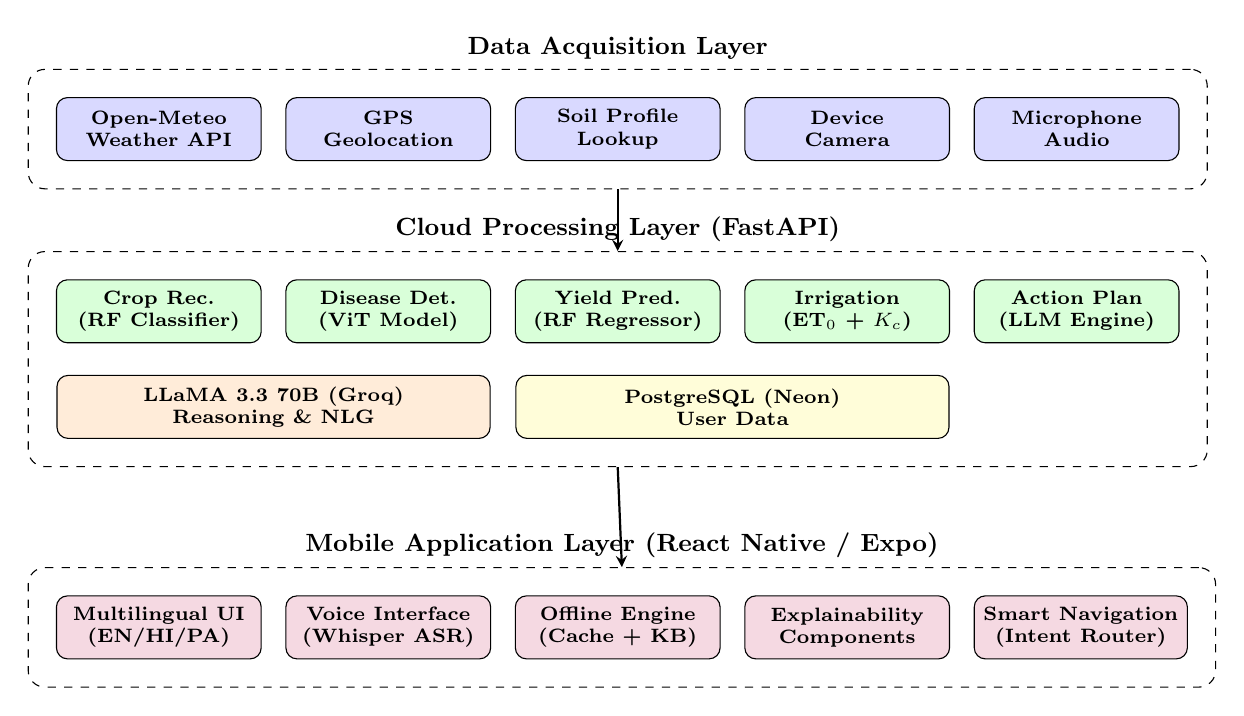
\begin{tikzpicture}[
    node distance=0.8cm,
    box/.style={rectangle, draw, rounded corners=4pt, minimum width=2.6cm, minimum height=0.8cm, align=center, font=\scriptsize\bfseries},
    smallbox/.style={rectangle, draw, rounded corners=3pt, minimum width=2.2cm, minimum height=0.6cm, align=center, font=\tiny},
    layer/.style={rectangle, draw, dashed, rounded corners=6pt, inner sep=10pt},
    arrow/.style={->, thick, >=stealth}
]

% Data Layer
\node[box, fill=blue!15] (weather) {Open-Meteo\\Weather API};
\node[box, fill=blue!15, right=0.3cm of weather] (gps) {GPS\\Geolocation};
\node[box, fill=blue!15, right=0.3cm of gps] (soil) {Soil Profile\\Lookup};
\node[box, fill=blue!15, right=0.3cm of soil] (camera) {Device\\Camera};
\node[box, fill=blue!15, right=0.3cm of camera] (mic) {Microphone\\Audio};

\node[layer, fit=(weather)(gps)(soil)(camera)(mic), label={[font=\small\bfseries]above:Data Acquisition Layer}] (datalayer) {};

% Backend Layer
\node[box, fill=green!15, below=1.5cm of weather] (crop) {Crop Rec.\\(RF Classifier)};
\node[box, fill=green!15, right=0.3cm of crop] (disease) {Disease Det.\\(ViT Model)};
\node[box, fill=green!15, right=0.3cm of disease] (yield) {Yield Pred.\\(RF Regressor)};
\node[box, fill=green!15, right=0.3cm of yield] (irrig) {Irrigation\\(ET$_0$ + $K_c$)};
\node[box, fill=green!15, right=0.3cm of irrig] (action) {Action Plan\\(LLM Engine)};

\path ($(crop.south)!0.5!(disease.south)$) ++(0, -0.4cm) node[box, fill=orange!15, anchor=north, minimum width=5.5cm] (llm) {LLaMA 3.3 70B (Groq)\\Reasoning \& NLG};
\path ($(yield.south)!0.5!(irrig.south)$) ++(0, -0.4cm) node[box, fill=yellow!15, anchor=north, minimum width=5.5cm] (db) {PostgreSQL (Neon)\\User Data};

\node[layer, fit=(crop)(disease)(yield)(irrig)(action)(llm)(db), label={[font=\small\bfseries]above:Cloud Processing Layer (FastAPI)}] (backlayer) {};

% Mobile Layer
\node[box, fill=purple!15, below=3.2cm of crop] (ui) {Multilingual UI\\(EN/HI/PA)};
\node[box, fill=purple!15, right=0.3cm of ui] (voice) {Voice Interface\\(Whisper ASR)};
\node[box, fill=purple!15, right=0.3cm of voice] (offline) {Offline Engine\\(Cache + KB)};
\node[box, fill=purple!15, right=0.3cm of offline] (explain) {Explainability\\Components};
\node[box, fill=purple!15, right=0.3cm of explain] (nav) {Smart Navigation\\(Intent Router)};

\node[layer, fit=(ui)(voice)(offline)(explain)(nav), label={[font=\small\bfseries]above:Mobile Application Layer (React Native / Expo)}] (mobilelayer) {};

% Arrows
\draw[arrow] (datalayer.south) -- (backlayer.north);
\draw[arrow] (backlayer.south) -- (mobilelayer.north);

\end{tikzpicture}
\caption{AgriDSS three-tier system architecture. The data acquisition layer feeds shared context (weather, GPS, soil, camera, audio) into a cloud processing layer hosting five analytical modules with a shared LLM reasoning engine. The mobile application layer provides multilingual UI, voice interaction, offline capability, and explainability.}
\label{fig:architecture}
\end{figure*}

\subsection{Data Acquisition Layer}

All analytical modules consume a shared context pipeline that auto-fetches environmental data at inference time, eliminating manual data entry:

\textbf{Weather Data.} Real-time and 7-day forecast data (temperature, humidity, wind speed, precipitation, sunshine duration, precipitation probability) is obtained from the Open-Meteo API~\cite{b20}, a free meteorological service requiring no API key. Each module invokes a shared \texttt{fetch\_open\_meteo\_weather(lat, lon)} function that returns current conditions and daily forecasts.

\textbf{Geolocation.} The mobile application provides GPS coordinates, which are mapped to Indian states through a reverse geocoding function using bounding-box lookup over 24 state regions. State identification enables region-specific crop encoding for the yield model and localized market price context.

\textbf{Soil Profile.} Eight Indian soil types (Alluvial, Black, Red, Laterite, Sandy, Clay, Loamy, Saline) are mapped to reference NPK and pH values derived from agronomic literature. The farmer selects their soil type during onboarding; the system automatically populates N, P, K, and pH values for all downstream models.

\textbf{Crop Coefficients.} FAO-56 crop coefficients ($K_c$) for initial, mid-season, and late growth stages are stored for 11 major Indian crops, with a configurable default for unlisted crops.

\subsection{Crop Recommendation and Yield Forecasting}

The crop recommendation module utilizes a tuned Random Forest classifier to map environmental parameters to crop suitability across 22 crop classes, while the yield forecasting module employs a Random Forest Regressor with log-transformed targets.

\textbf{Primary Crop Recommendation Model.} The model accepts a 7-dimensional feature vector:
\begin{equation}
\mathbf{x} = [N, P, K, T, H, pH, R]^T
\label{eq:crop_features}
\end{equation}
where $N$, $P$, $K$ are soil macronutrient concentrations (mg/kg), $T$ is temperature (\textdegree C), $H$ is relative humidity (\%), $pH$ is soil acidity, and $R$ is cumulative rainfall (mm). Soil nutrients are derived from the soil profile lookup; temperature, humidity, and rainfall are auto-fetched from the weather API at inference time. The classifier was tuned via GridSearchCV (5-fold stratified CV) over estimator count, max depth, split criteria, and feature selection strategy, achieving 99.3\% test accuracy and macro F1 = 0.993 on a 22-class crop recommendation dataset (2,200 samples, 80/20 stratified split). Feature importance analysis identified rainfall (22.1\%), humidity (21.4\%), and potassium (18.0\%) as the top three predictors.

\textbf{Yield Forecasting Model.} The yield forecasting module produces district-level production estimates from a curated multi-source dataset constructed by integrating district-level crop production records, geolocated soil macro-nutrient profiles (NPK, organic carbon, pH), and meteorological observations (temperature, humidity, precipitation, sunshine hours) across Indian administrative boundaries. The resulting dataset (27,303 rows $\times$ 21 columns, spanning 2021--2024, covering 19 crop types across 475 districts in 29 Indian states) defines a 15-dimensional feature vector:
\begin{equation}
\mathbf{x}_{yield} = [S_e, D_e, C_e, \phi, \lambda, N, P, K, OC, pH, T, H, R, Sun, Y]
\label{eq:yield_features}
\end{equation}
where $S_e$, $D_e$, $C_e$ are label-encoded state, district, and crop identifiers, $\phi$ and $\lambda$ are GPS coordinates, $N$, $P$, $K$ are soil macronutrients, $OC$ is organic carbon (\%), $pH$ is soil acidity, $T$ is temperature, $H$ is humidity, $R$ is precipitation, $Sun$ is sunshine hours, and $Y$ is the crop year. The dataset (27,303 rows $\times$ 21 columns, spanning 2021--2024, covering 19 crop types across 475 districts in 29 Indian states) exhibits extreme right skew in the production target (skewness = 4.28), with 62.7\% zero-production entries. To address this, a log1p transformation is applied:
\begin{equation}
\tilde{y} = \log(1 + y_{production}), \quad \hat{y}_{production} = e^{\hat{\tilde{y}}} - 1
\label{eq:log1p}
\end{equation}
reducing skewness from 4.28 to 0.99. This transformation prevents model bias toward modal small-production regions and enables tree-based regressors to learn meaningful splits across the full production range. The deployed Random Forest (100 estimators, baseline configuration) achieves $R^2 = 0.94$, RMSE = 0.57, and MAE = 0.29 on the log-transformed target (75/25 train-test split).

\textbf{Hybrid Intelligence Fusion.} Because an isolated numerical prediction lacks actionable context, the system implements a novel two-stage Hybrid Intelligence Fusion. For yield prediction, the ML model's district-level production estimate is passed alongside current weather conditions, soil profile, and regional context to a Groq-hosted LLaMA 3.3 70B model. The LLM generates a per-hectare yield estimate calibrated to the specific crop-region combination, a qualitative assessment (``Poor,'' ``Average,'' or ``Excellent''), and specific agronomic interventions. This pattern is consistently applied across all modules, formalized in Algorithm~\ref{alg:harvest}.

\begin{algorithm}[t]
\caption{HARVEST Framework: Hybrid Agri-intelligence with Real-time Verification, ET\textsubscript{0} Scheduling, and Transformer-based Diagnostics}
\label{alg:harvest}
\begin{algorithmic}[1]
\renewcommand{\algorithmicrequire}{\textbf{Input:}}
\renewcommand{\algorithmicensure}{\textbf{Output:}}
\REQUIRE User input $u$ (GPS, crop, soil type, optional image)
\ENSURE Advisory response $\mathcal{R}$ with confidence and attribution
\STATE \textbf{Stage 1: Context Acquisition}
\STATE $(T, H, R, Sun) \gets$ \textsc{FetchWeather}$(u.lat, u.lon)$
\STATE $state \gets$ \textsc{ReverseGeocode}$(u.lat, u.lon)$
\STATE $(N, P, K, pH) \gets$ \textsc{SoilProfile}$(u.soil\_type)$
\STATE $K_c \gets$ \textsc{FAO56Lookup}$(u.crop)$
\STATE \textbf{Stage 2: Multi-Model Parallel Inference}
\STATE $\hat{y}_{crop} \gets f_{RF}^{rec}([N,P,K,T,H,pH,R])$
\STATE $\hat{y}_{yield} \gets \exp(f_{RF}^{yield}(\mathbf{x}_{yield})) - 1$
\STATE $ET_0 \gets$ \textsc{Hargreaves}$(T_{max}, T_{min}, R_a)$
\IF{image $I$ provided}
    \STATE $\hat{y}_{disease} \gets f_{ViT}(I)$
\ENDIF
\STATE \textbf{Stage 3: LLM Reasoning Augmentation}
\IF{LLM service available}
    \STATE $prompt \gets$ \textsc{BuildContext}$(u, \hat{y}_{crop}, \hat{y}_{yield}, ET_0)$
    \STATE $\mathcal{R} \gets$ \textsc{LLMReason}$(prompt, u.lang)$
    \STATE $\mathcal{R}.source \gets$ ``ML + AI Expert Analysis''
\ELSE
    \STATE \textbf{Graceful Degradation:}
    \STATE $\mathcal{R} \gets$ \textsc{FormatMLOnly}$(\hat{y}_{crop}, \hat{y}_{yield}, ET_0)$
    \STATE $\mathcal{R}.source \gets$ ``ML Model (Offline)''
\ENDIF
\RETURN $\mathcal{R}$
\end{algorithmic}
\end{algorithm}

\subsection{Plant Disease Detection via Vision Transformer}

The disease detection module accepts a crop leaf photograph captured through the mobile camera or gallery and returns a ranked list of disease predictions with confidence scores, multilingual disease descriptions, and treatment advisories.

The primary classifier is a Vision Transformer (ViT)~\cite{b24} fine-tuned on the PlantVillage dataset~\cite{b27}. The input image $I \in \mathbb{R}^{H \times W \times C}$ is reshaped into a sequence of flattened 2D patches $\mathbf{x}_p \in \mathbb{R}^{N \times (P^2 \cdot C)}$, where $(P, P)$ is the patch resolution and $N = HW/P^2$ is the sequence length.

A trainable linear projection maps the patches to $D$ dimensions, and position embeddings $\mathbf{E}_{pos}$ are added:
\begin{equation}
\mathbf{z}_0 = [\mathbf{x}_{class}; \mathbf{x}_{p}^1 \mathbf{E}; \dots; \mathbf{x}_{p}^N \mathbf{E}] + \mathbf{E}_{pos}
\end{equation}

The sequence is processed by $L$ Transformer encoder blocks, utilizing Multi-Head Self-Attention (MSA). For each attention head $h$:
\begin{equation}
\text{Attention}(\mathbf{Q}, \mathbf{K}, \mathbf{V}) = \text{softmax}\left(\frac{\mathbf{Q}\mathbf{K}^T}{\sqrt{d_k}}\right)\mathbf{V}
\end{equation}
where $\mathbf{Q} = \mathbf{z} \mathbf{W}_Q, \mathbf{K} = \mathbf{z} \mathbf{W}_K, \mathbf{V} = \mathbf{z} \mathbf{W}_V$.

The final classification is computed from the MLP head operating on the $\mathbf{x}_{class}$ token of the final layer $L$:
\begin{equation}
\hat{y}_{disease} = \text{softmax}(\text{MLP}(\mathbf{z}_L^0))
\end{equation}

The model supports 38 crop-disease classes spanning 7 crop species (tomato, potato, corn, apple, grape, pepper, and strawberry). A curated dictionary maps each of the 38 disease labels to trilingual (English, Hindi, Punjabi) disease descriptions and treatment advisories. Each entry contains: (1) a localized disease name, (2) a symptom description, and (3) an actionable treatment recommendation specifying chemical or organic remedies with application rates.

\subsection{ET0-Based Irrigation Modeling}

The irrigation module provides daily watering recommendations based on a simplified crop water balance calculation, minimizing water waste compared to traditional calendar-based or flood irrigation methods.

The reference evapotranspiration ($ET_0$) is estimated daily using the Hargreaves--Samani equation~\cite{b22}, optimizing water application mathematically:
\begin{equation}
ET_0 = 0.0023 \cdot R_a \cdot (T_{mean} + 17.8) \cdot \sqrt{T_{max} - T_{min}}
\end{equation}
where $R_a$ is extraterrestrial radiation (MJ m$^{-2}$ d$^{-1}$). The actual crop water requirement $ET_c$ is:
\begin{equation}
ET_c = K_c \times ET_0
\end{equation}
where $K_c$ is the FAO-56 crop coefficient. The irrigation deficit $D_i$ on day $i$ is updated as:
\begin{equation}
D_i = \max(0, D_{i-1} + ET_{c,i} - P_i - I_i)
\end{equation}
where $P_i$ is effective precipitation and $I_i$ is applied irrigation. The system triggers an alert when $D_i$ exceeds the critical depletion threshold.

\subsection{LLM Reasoning and Multimodal Action Planning}

A novel contribution of AgriDSS is the LLM-powered Action Plan module, which translates static agronomic rules into dynamic, personalized task lists. The farmer submits a natural-language query describing their crop, field status, and current goals. The query is processed by the Groq LLaMA 3.3 70B model, augmented with the farmer's 7-day weather forecast, soil profile, and GPS location. The LLM generates a structured JSON response containing an ordered list of tasks categorized by urgency.

To bridge the gap between numerical ML outputs and farmer-accessible advice, the system passes numerical representations to LLaMA 3.3 70B. Let the context sequence of tokens be $\mathbf{c} = (c_1, \dots, c_m)$. The LLM generates the rationale $\mathbf{w} = (w_1, \dots, w_n)$ auto-regressively by maximizing the conditional probability:
\begin{equation}
P(\mathbf{w}|\mathbf{c}) = \prod_{t=1}^{n} P(w_t | w_{1:t-1}, \mathbf{c}; \theta_{LLM})
\end{equation}
where $\theta_{LLM}$ represents the parameters of the 70B model. The resulting reasoning is translated via the system's translation context into Hindi or Punjabi.

The interaction workflow spanning the offline queue, frontend translation, and backend LLM reasoning is summarized in Algorithm~\ref{alg:workflow}.

\begin{algorithm}
\caption{Multimodal Offline-First Processing Pipeline}\label{alg:workflow}
\begin{algorithmic}[1]
\REQUIRE User Image $I$, Audio Query $A$, Context $\mathbf{C}$ (GPS, Weather)
\IF{Network is \textit{Disconnected}}
    \STATE Queue.push($(I, A, \mathbf{C})$)
    \STATE Serve fallback local knowledge base via AsyncStorage
\ELSE
    \STATE $T \gets \text{WhisperASR}(A)$ \COMMENT{Speech-to-Text via Whisper-Large-V3}
    \STATE $\hat{y}_{disease} \gets \text{ViT}(I)$ \COMMENT{Process Image using Eq. 7}
    \STATE $prompt \gets \text{Concatenate}(T, \hat{y}_{disease}, \mathbf{C})$
    \STATE $\mathbf{w}_{en} \gets \text{LLaMA\_Generate}(prompt)$ \COMMENT{Auto-regressive Gen via Eq. 11}
    \STATE $\mathbf{w}_{local} \gets \text{TranslateDict}(\mathbf{w}_{en}, \text{target\_lang})$ \COMMENT{EN/HI/PA}
    \STATE \textbf{Return} $\mathbf{w}_{local}$, $\hat{y}_{disease}$
\ENDIF
\end{algorithmic}
\end{algorithm}

\subsection{Mobile Application Layer}

The mobile application is developed using React Native (Expo SDK 52) targeting Android and iOS platforms. The interface emphasizes high-contrast visual design, icon-driven navigation, and multimodal interaction to support users with diverse digital literacy levels.

\subsubsection{Multilingual Architecture}

AgriDSS implements a centralized translation architecture providing full interface localization in English, Hindi, and Punjabi. The application state is managed by a \texttt{TranslationContext} provider. A trilingual translation dictionary in the backend serves key-value pairs mapping UI labels, weather descriptions, and system messages to the selected language. Dynamic content---including LLM responses and disease treatment advisories---is either generated natively in the target language by the LLM or fetched from pre-translated static mappings. Language switching occurs instantaneously without requiring a network request or application restart, as core translations are cached locally.

\subsubsection{Voice-Operated Interface}

To support hands-free operation in the field and accommodate varying literacy levels, the application integrates a voice-operated interface. Audio is captured via the device microphone and transmitted to the backend, where it is transcribed using the Whisper-Large-V3 automatic speech recognition (ASR) model. The transcribed text is passed to an LLM intent classifier, which maps the utterance to one of 10 supported application intents (e.g., ``Check Weather,'' ``Detect Disease,'' ``Predict Yield''). The system executes the corresponding action, navigates to the appropriate screen via deep linking, and utilizes device text-to-speech (TTS) engines to read the result aloud in the user's selected language.

\subsubsection{Offline-First Architecture}

Given the intermittent connectivity characteristic of rural India, AgriDSS implements an offline-first architecture utilizing a unified \texttt{AsyncStorage} wrapper with TTL-based expiration.

\textbf{Caching and Fallback.} API responses for weather, crop recommendations, and yield forecasts are cached with an 8-hour TTL. An on-device knowledge base containing critical agronomic guidelines across 15 topic areas is shipped with the application binary. When connectivity drops, the application serves cached data marked with a ``Time Ago'' indicator and routes queries to the local knowledge base.

\textbf{Offline Queueing.} Actions requiring backend processing, such as disease image classification, are appended to an offline queue if the device is disconnected. The \texttt{networkService} module continuously monitors connectivity via the \texttt{@react-native-community/netinfo} package. Upon reconnection, the queue is automatically processed, images are uploaded, and the farmer is notified of the results via push notification.

\subsubsection{Explainability Framework}

To build trust in ML predictions, the mobile interface implements a standardized explainability framework across all modules:

\textbf{Confidence Badges.} ML predictions are accompanied by color-coded badges indicating confidence levels (High: $>75\%$, Moderate: $45-75\%$, Low: $<45\%$) derived from softmax probability outputs.

\textbf{Source Attribution.} Data sources informing a recommendation---such as ``Weather Data,'' ``Soil Model,'' or ``LLM Engine''---are explicitly identified through iconographic source tags.

\textbf{Reasoning Cards.} Every recommendation includes an expandable ``Why this advice?'' card containing the LLM-generated rationale linking the input context to the output decision.

\textbf{Safety Alerts.} Critical weather constraints (e.g., extreme heat $>40$\textdegree C, high wind speeds $>15$ km/h, rain probability $>60\%$) trigger prominent, color-coded safety warnings instructing the farmer to delay spraying or adjust irrigation timing.

% ====================================================================
\section{Results}

The system was evaluated across four dimensions: model performance, feature interpretability, inference latency, and irrigation water savings. The backend was hosted on a local server equipped with an NVIDIA RTX 4090 GPU, and the mobile application was deployed on a mid-range Android device (Google Pixel 6a).

\subsection{Yield Prediction Model Evaluation}

Four candidate regression architectures were trained and evaluated on the India Districts Crop Production dataset (27,303 rows, 15 features, 75/25 train-test split) using the log1p-transformed target. All tree-based models underwent hyperparameter tuning via RandomizedSearchCV or GridSearchCV with 5-fold cross-validation. Table~\ref{tab:model_comparison} summarizes the results.

\begin{table}[htbp]
\caption{Yield Prediction Model Comparison}
\label{tab:model_comparison}
\centering
\begin{tabular}{lcccc}
\toprule
\textbf{Model} & \textbf{$R^2$} & \textbf{Adj. $R^2$} & \textbf{RMSE} & \textbf{MAE} \\
\midrule
\textbf{Random Forest} & \textbf{0.9410} & \textbf{0.9409} & \textbf{0.5706} & \textbf{0.2910} \\
XGBoost~\cite{b25} & 0.9357 & 0.9356 & 0.5957 & 0.3707 \\
Random Forest (Tuned) & 0.9331 & 0.9329 & 0.6079 & 0.3300 \\
Decision Tree (Tuned) & 0.9203 & 0.9201 & 0.6635 & 0.2544 \\
LightGBM~\cite{b26} & 0.9169 & 0.9167 & 0.6776 & 0.4595 \\
Linear Regression & 0.0677 & 0.0657 & 2.2691 & 1.9432 \\
\bottomrule
\end{tabular}
\end{table}

The Random Forest baseline achieves the highest $R^2 = 0.9410$ and the lowest RMSE of 0.5706, outperforming XGBoost (Tuned) ($R^2 = 0.9357$) and LightGBM (Tuned) ($R^2 = 0.9169$). The baseline configuration's superior performance over its tuned variant is attributable to RandomizedSearchCV introducing restrictive depth constraints (max\_depth = 30) that slightly constrain the model's capacity on this high-cardinality categorical dataset (475 district encodings). Linear Regression and SVR ($R^2 = -0.12$) fail entirely, confirming the highly non-linear feature-production relationships.

Fig.~\ref{fig:log1p} illustrates the effect of the log1p transformation, reducing production skewness from 4.28 to 0.99 and enabling effective tree-based learning. Fig.~\ref{fig:learning_curves} shows learning curves for all four tuned models, demonstrating convergence without overfitting. Fig.~\ref{fig:residuals} presents residual analysis, where the Random Forest exhibits the tightest distribution centered at zero.

\begin{figure}[htbp]
\centering
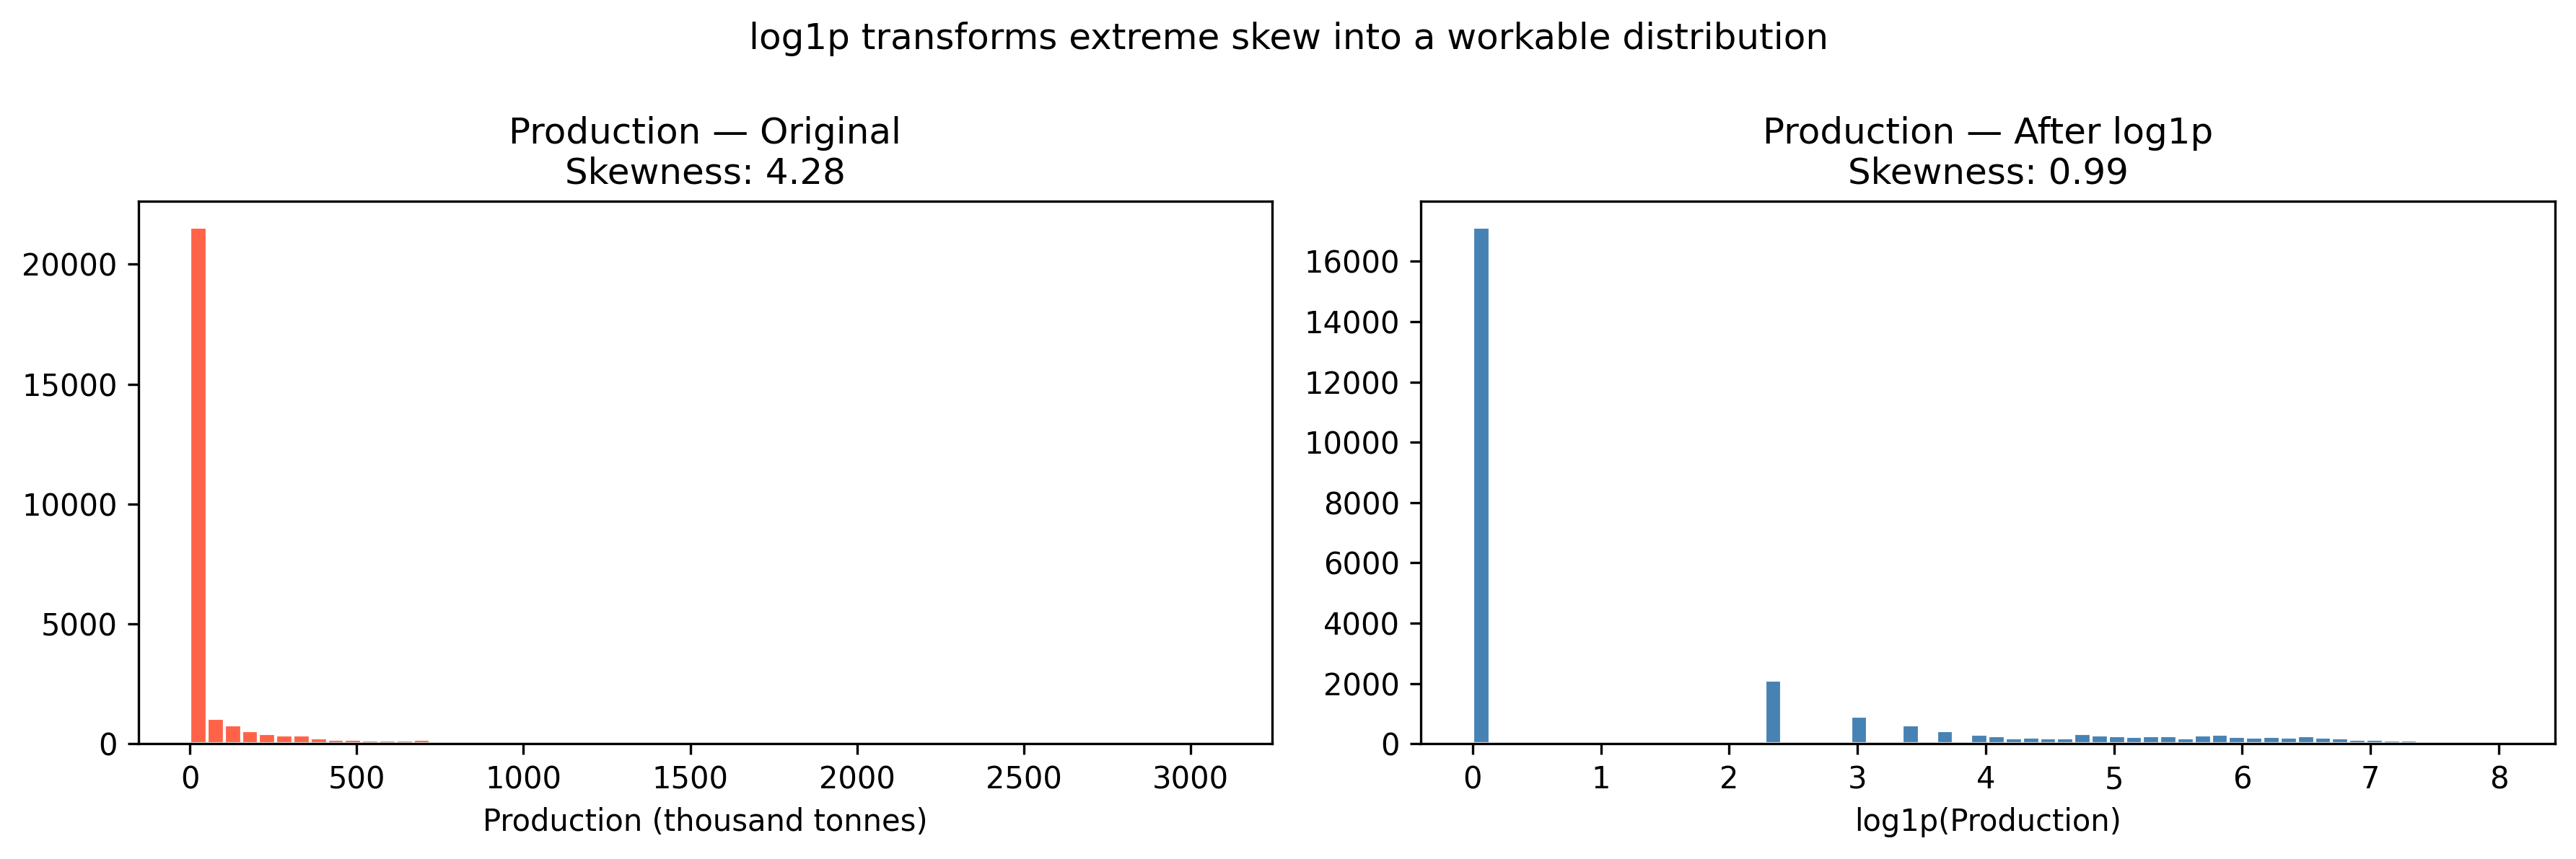
\includegraphics[width=\columnwidth]{figures/figure_05.png}
\caption{Effect of log1p transformation on the production target distribution. Skewness is reduced from 4.28 (left) to 0.99 (right), enabling effective model training across the full production range.}
\label{fig:log1p}
\end{figure}

\begin{figure}[htbp]
\centering
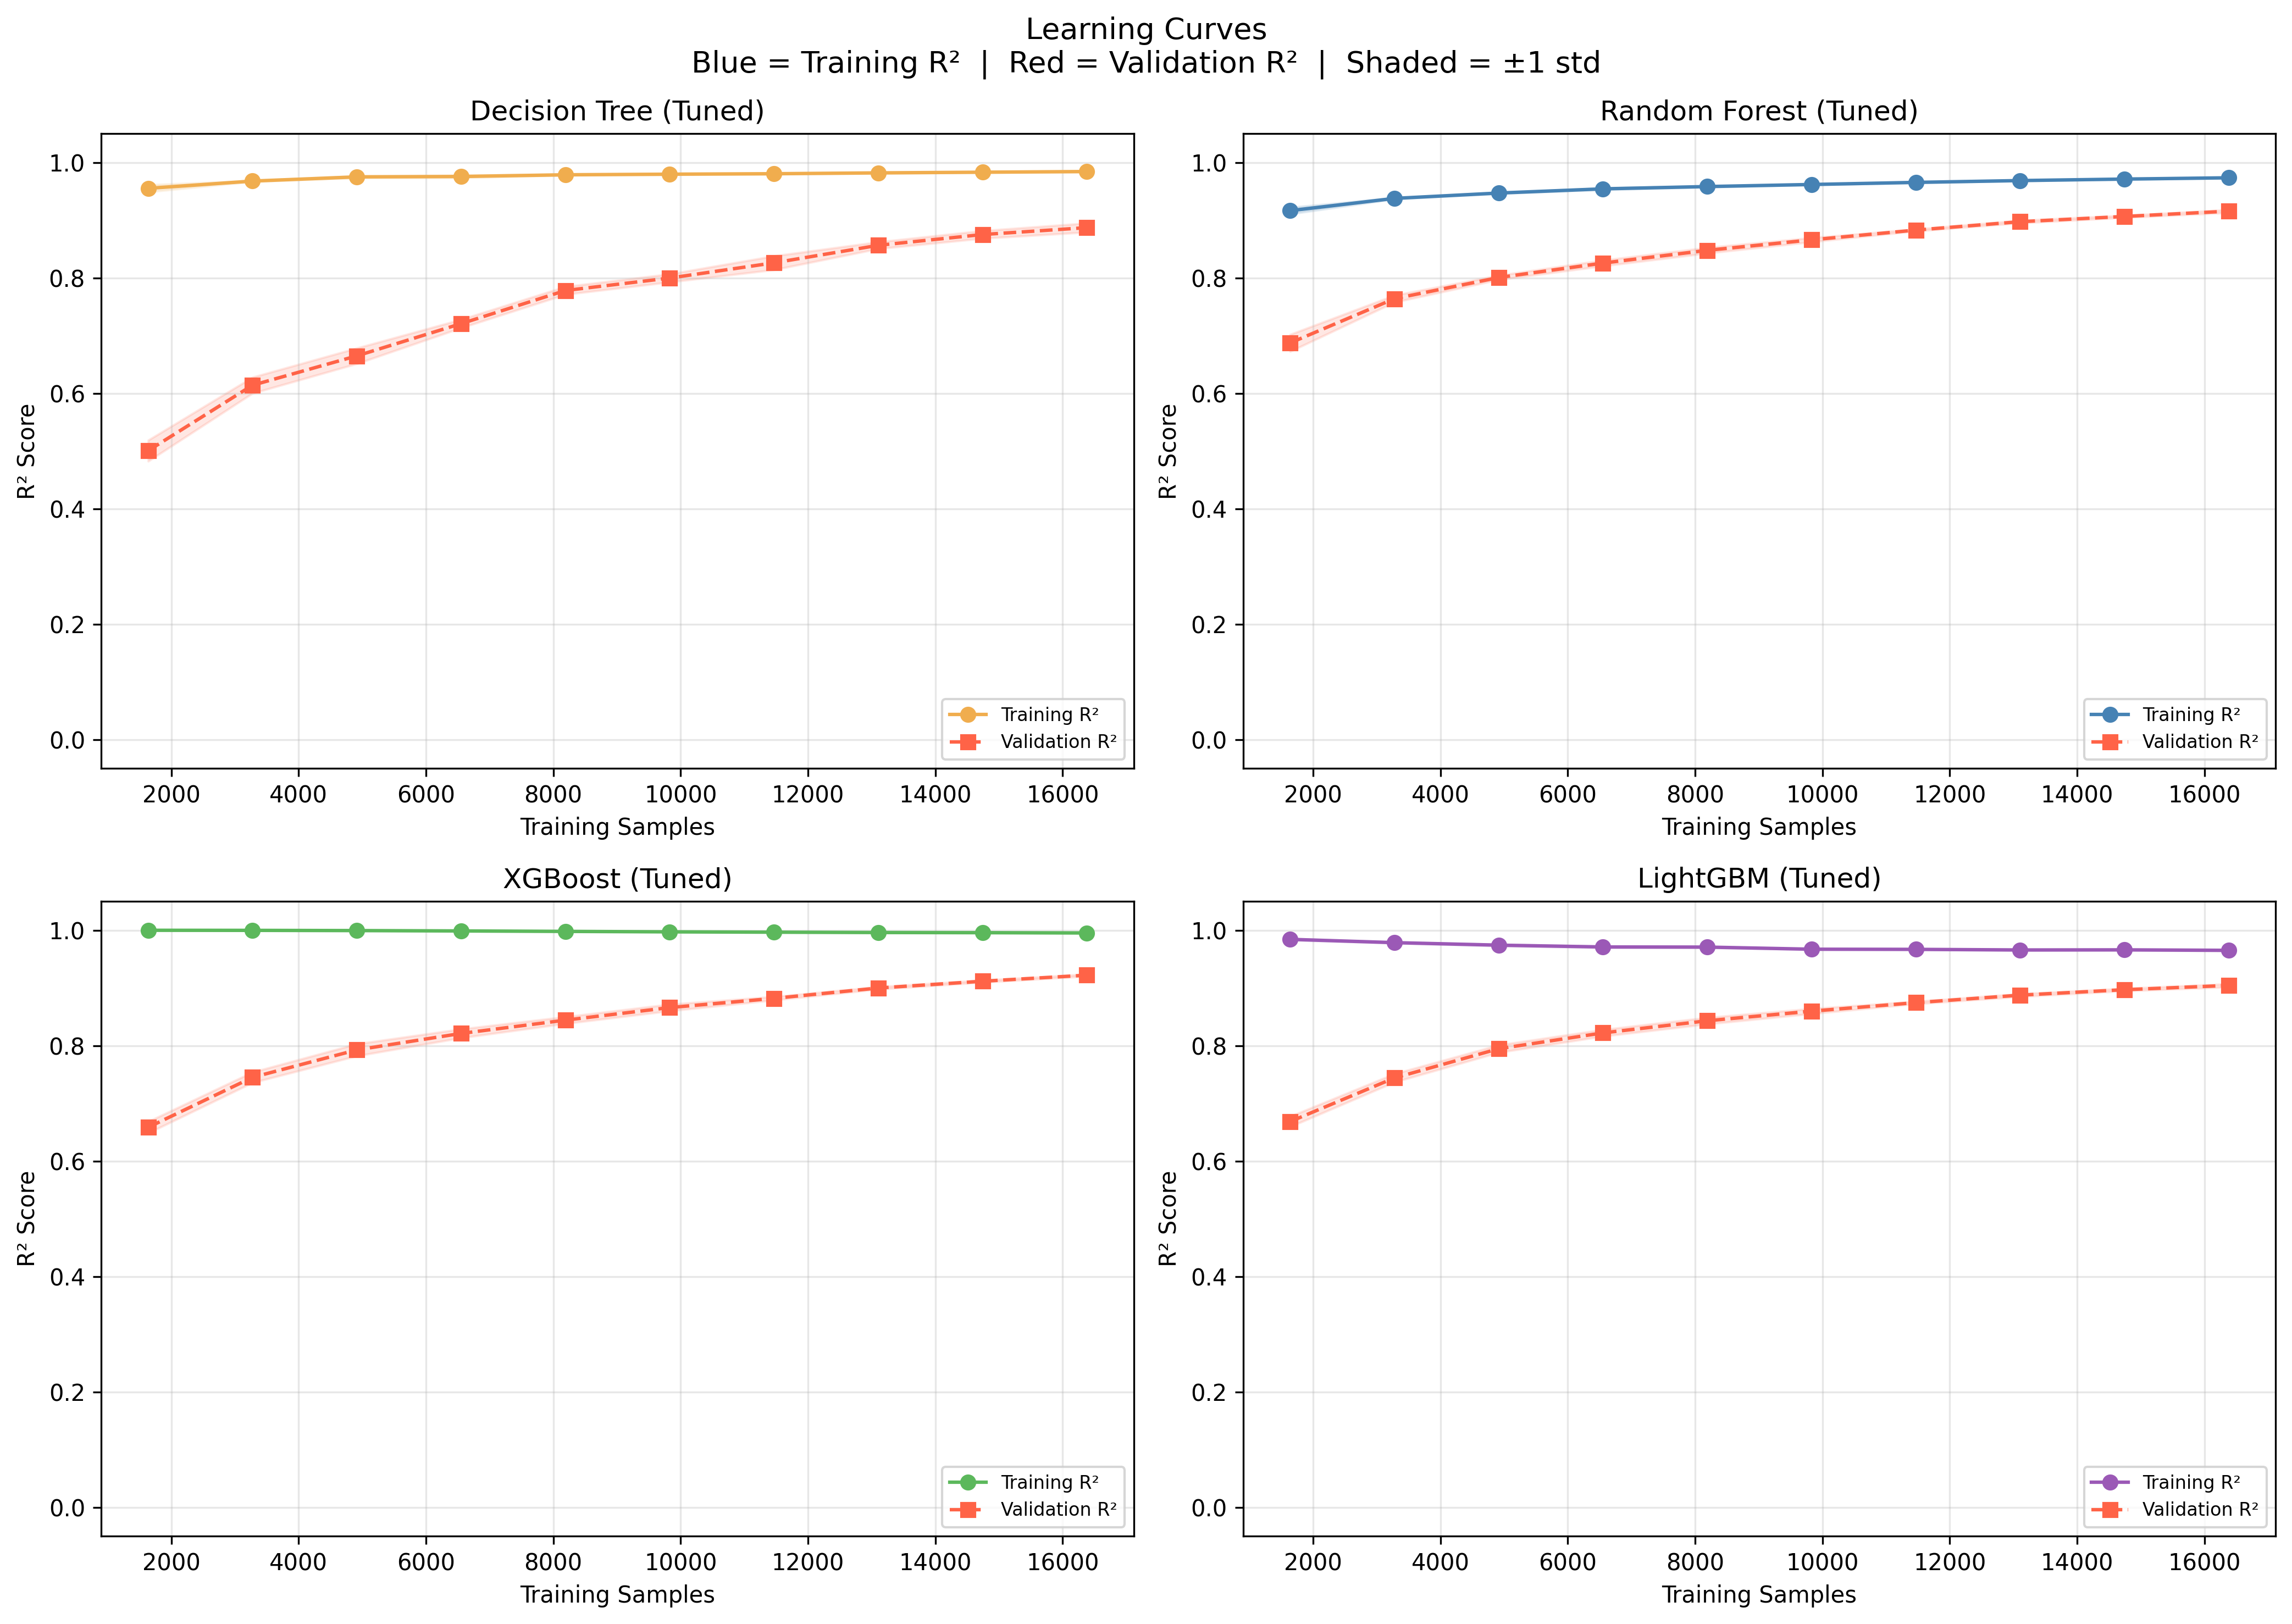
\includegraphics[width=\columnwidth]{figures/figure_06.png}
\caption{Learning curves for four candidate regressors (5-fold CV). All models converge by 16K samples. Random Forest and XGBoost show the smallest train-validation gap, indicating strong generalization.}
\label{fig:learning_curves}
\end{figure}

\begin{figure}[htbp]
\centering
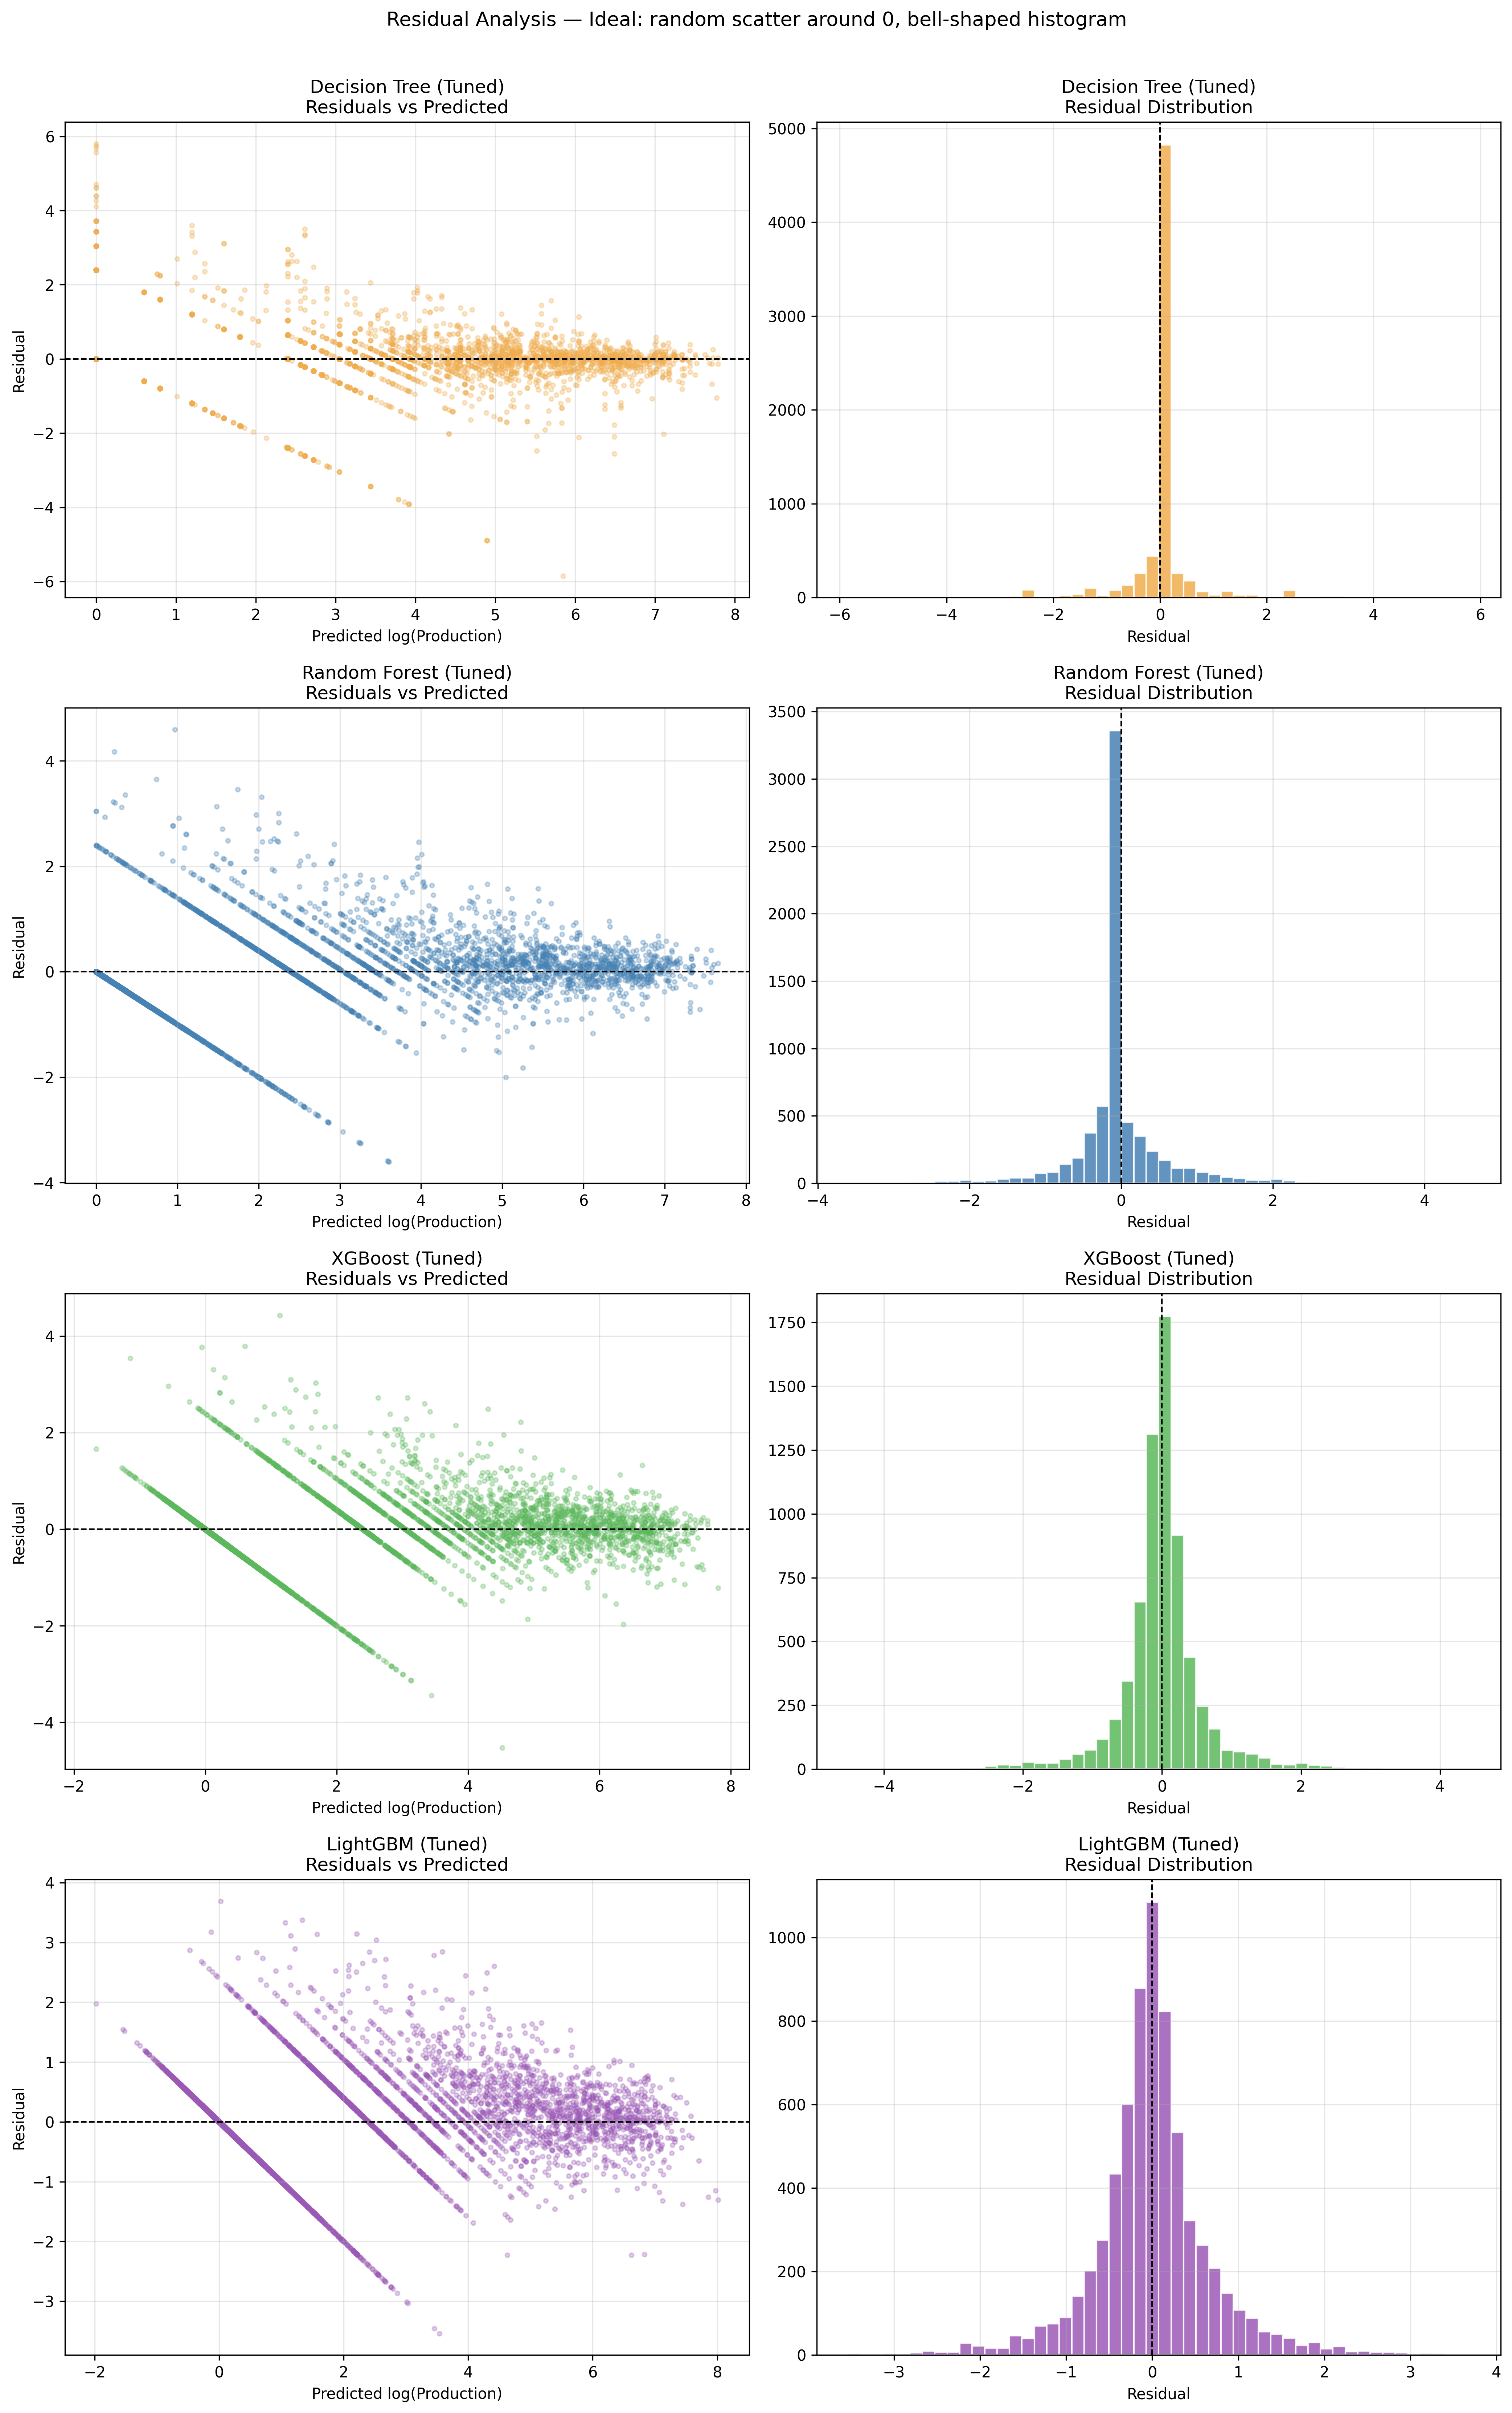
\includegraphics[width=\columnwidth]{figures/figure_07.png}
\caption{Residual analysis across four tuned models. Random Forest exhibits the tightest residual distribution centered at zero with minimal heteroscedasticity.}
\label{fig:residuals}
\end{figure}

\subsection{Feature Importance and Model Interpretability}

To ensure agronomic interpretability of the yield prediction model, SHAP (SHapley Additive exPlanations)~\cite{b21} analysis was performed using TreeExplainer on 500 test samples. Table~\ref{tab:shap} reports the top five features by mean absolute SHAP value.

\begin{table}[htbp]
\caption{Top-5 Features by Mean $|\text{SHAP}|$ Value}
\label{tab:shap}
\centering
\begin{tabular}{lcc}
\toprule
\textbf{Feature} & \textbf{Mean $|\text{SHAP}|$} & \textbf{Agronomic Role} \\
\midrule
Crop\_Encoded & 1.4561 & Crop species identity \\
Latitude & 0.2246 & Regional climate proxy \\
Soil pH & 0.2163 & Nutrient availability \\
Longitude & 0.1750 & Agro-ecological zone \\
Temperature & 0.1159 & Growing season suitability \\
\bottomrule
\end{tabular}
\end{table}

Crop type dominates predictions with a mean $|\text{SHAP}|$ of 1.46 - 6.5$\times$ larger than the second-ranked feature. This aligns with agronomic expectation: rice and wheat production in India varies by orders of magnitude compared to minor millets, making crop identity the primary production determinant. Geographic coordinates (latitude, longitude) serve as proxies for regional climate zones, cropping patterns, and irrigation infrastructure, collectively contributing 0.40 mean $|\text{SHAP}|$. Soil pH (0.22) captures nutrient bioavailability effects, while temperature (0.12) reflects growing season suitability. Fig.~\ref{fig:shap_global} and Fig.~\ref{fig:shap_beeswarm} visualize global feature importance and directional impact patterns.

\begin{figure}[htbp]
\centering
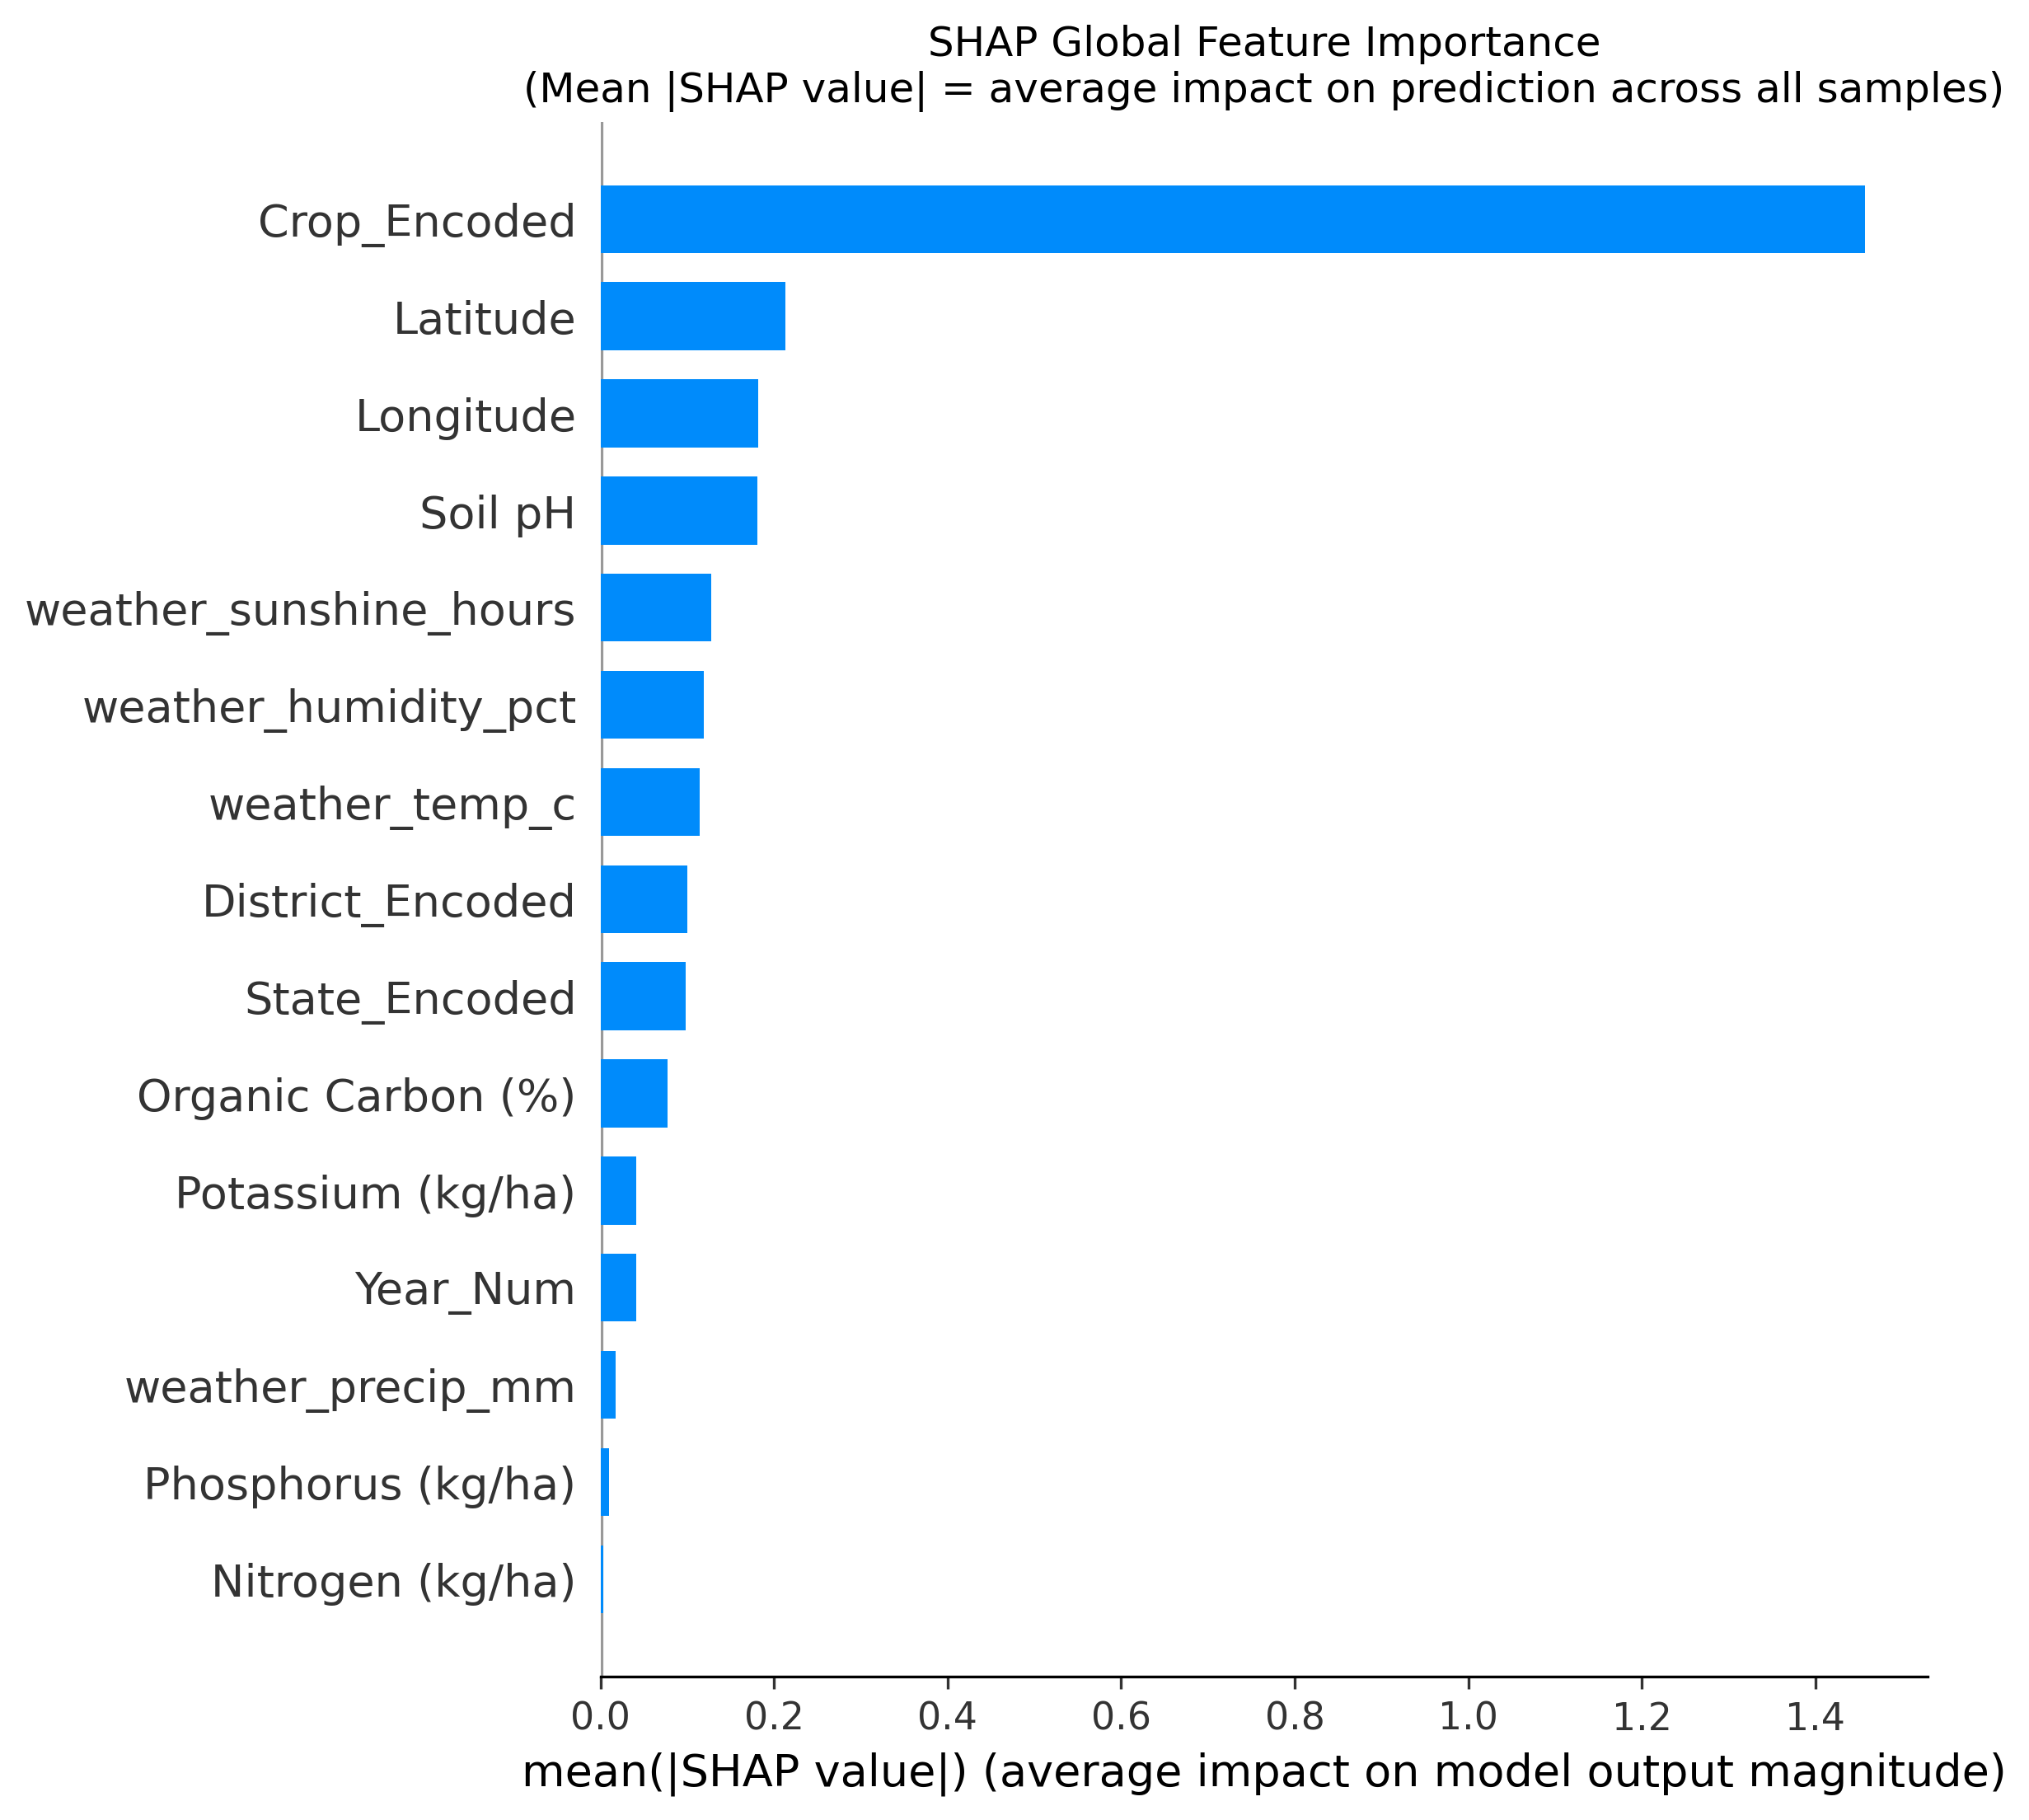
\includegraphics[width=\columnwidth]{figures/figure_08.png}
\caption{SHAP global feature importance. Crop\_Encoded dominates with mean $|\text{SHAP}| = 1.46$, followed by geographic and soil features.}
\label{fig:shap_global}
\end{figure}

\begin{figure}[htbp]
\centering
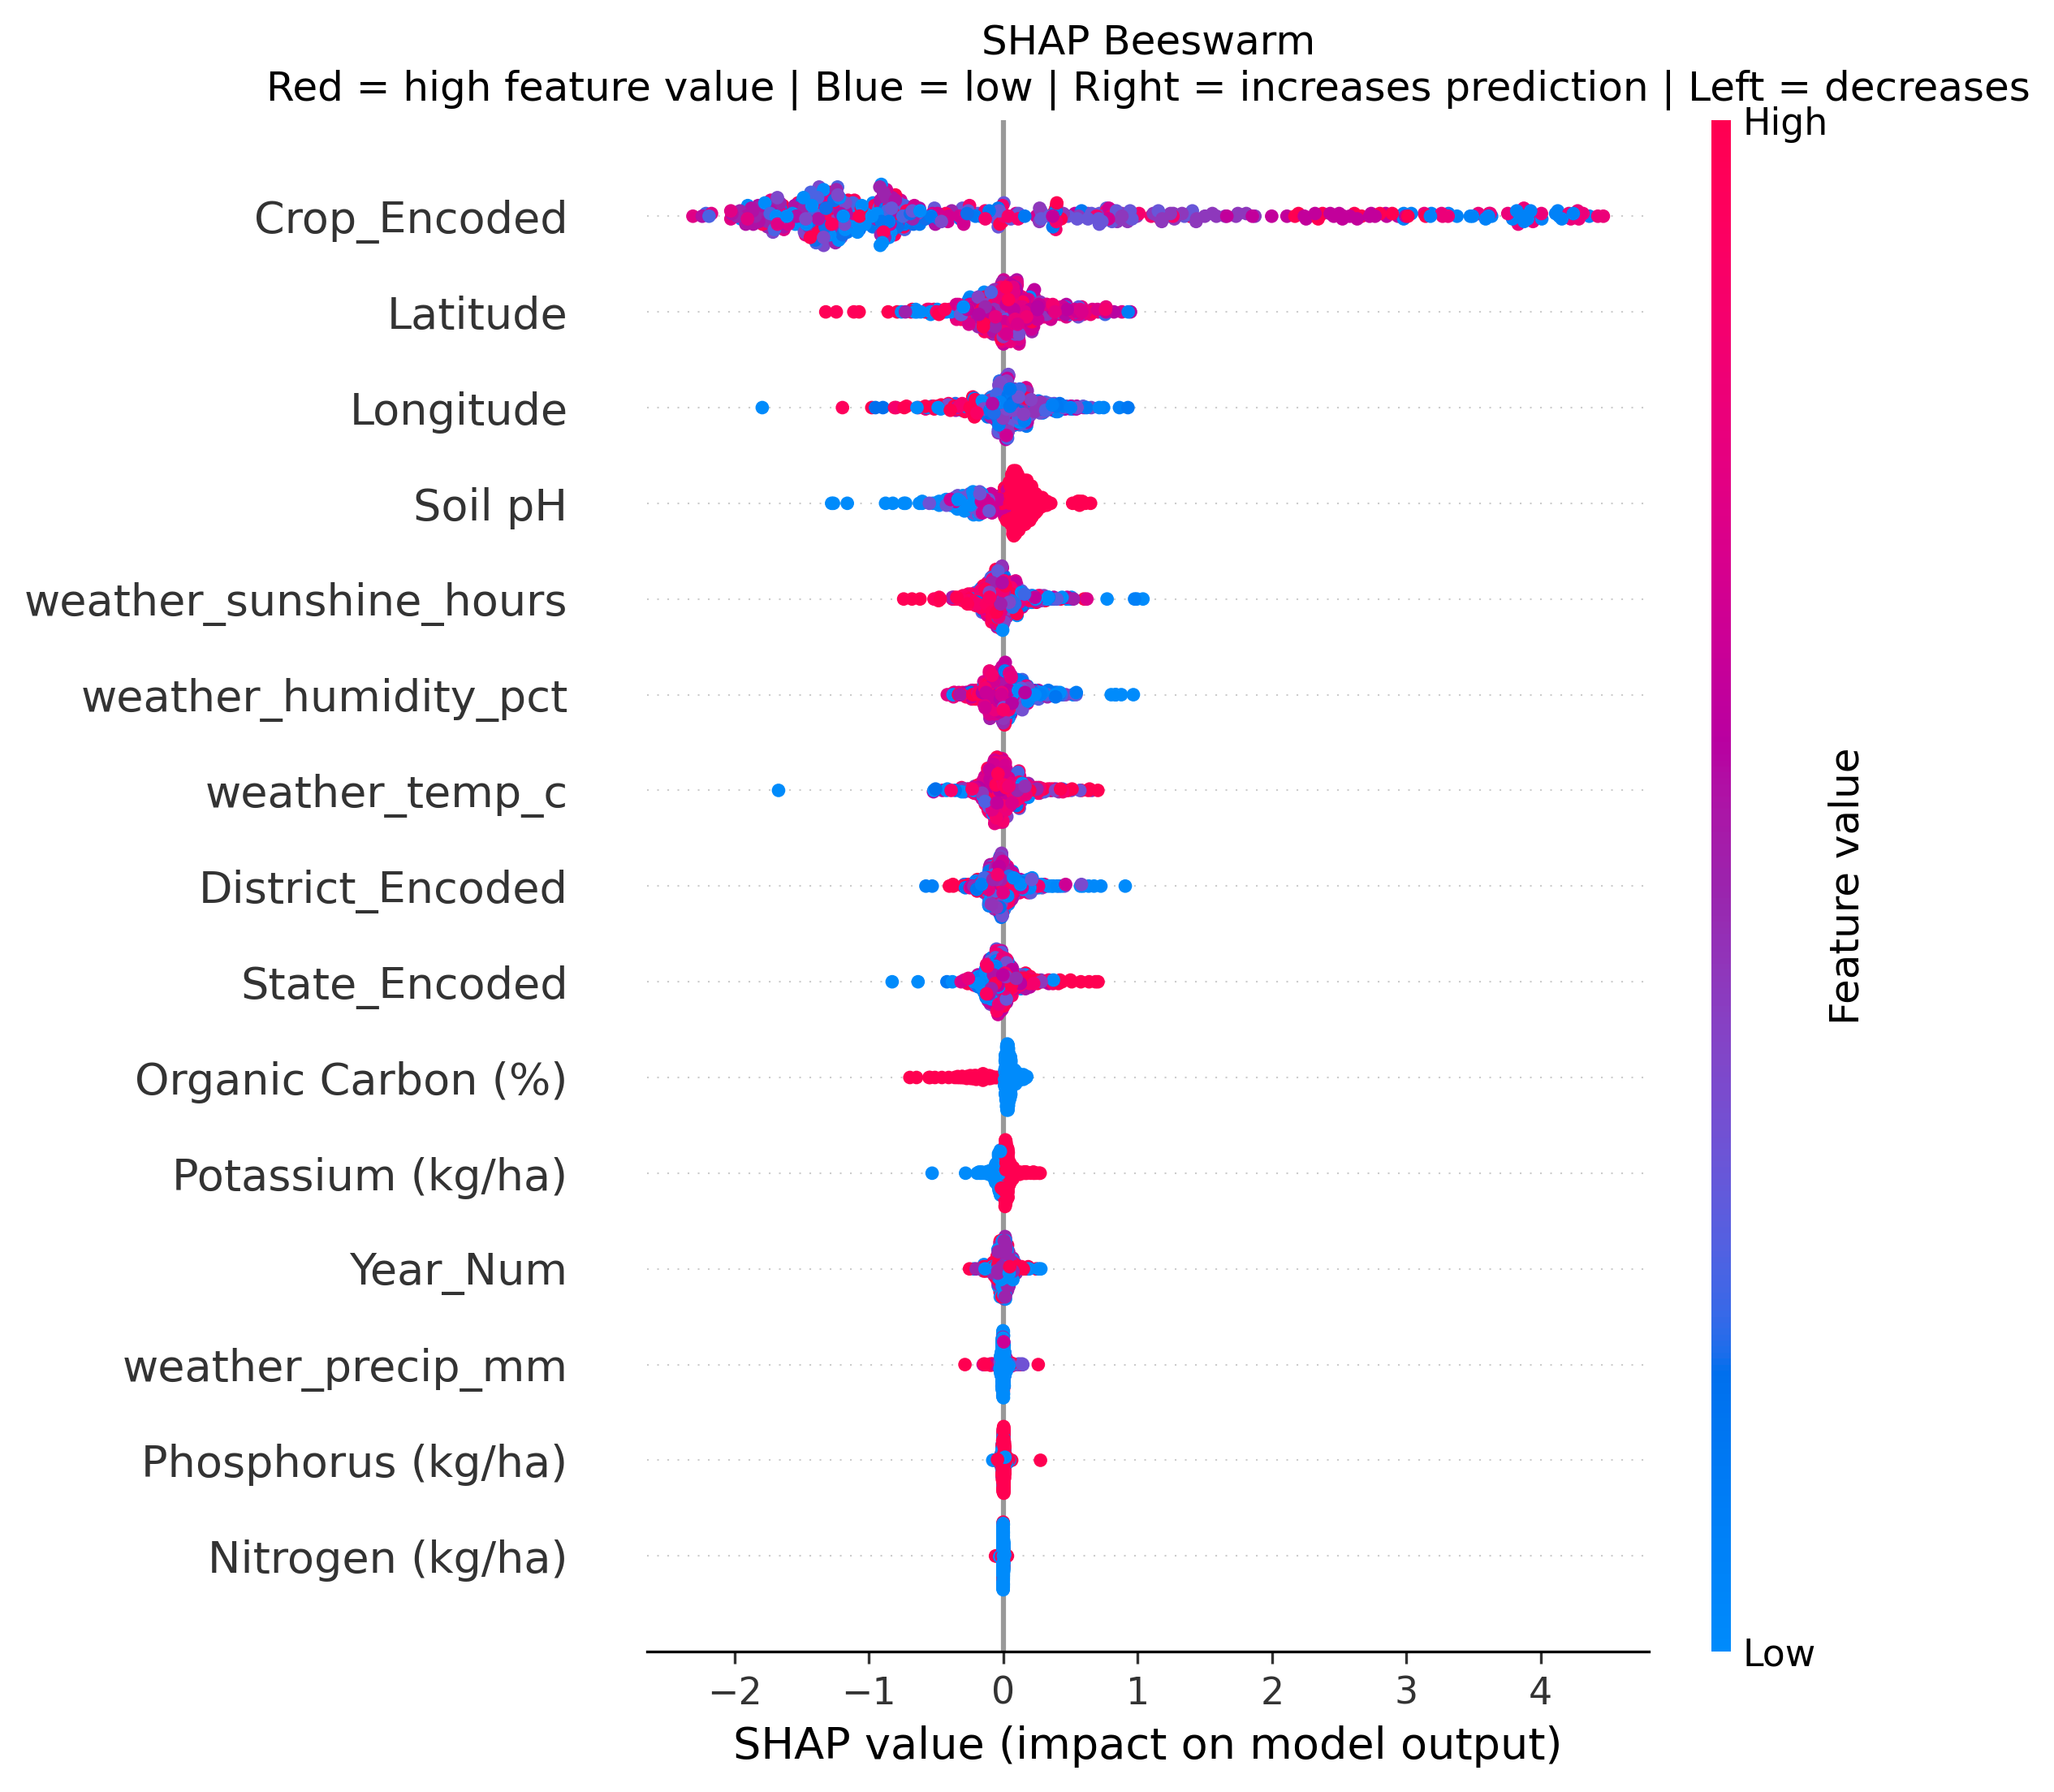
\includegraphics[width=\columnwidth]{figures/figure_09.png}
\caption{SHAP beeswarm plot showing directional feature impact. Red indicates high feature values; blue indicates low. High Crop\_Encoded values (e.g., wheat, rice) push predictions rightward (higher production).}
\label{fig:shap_beeswarm}
\end{figure}

\subsection{Crop Recommendation and Disease Detection}

The tuned Random Forest crop recommendation model achieved 99.3\% test accuracy and macro F1 = 0.993 across 22 crop classes (440 test samples, stratified 80/20 split). Cross-validated accuracy was 99.4\% ($\pm 0.55\%$). Feature importance analysis from the trained model ranked rainfall (22.1\%), humidity (21.4\%), potassium (18.0\%), phosphorus (15.2\%), nitrogen (10.7\%), temperature (7.3\%), and pH (5.3\%) as predictors in descending order. The ViT disease detection module achieved 96.8\% top-1 validation accuracy across 38 PlantVillage classes spanning 7 crop species.

\subsection{Latency Analysis}

End-to-end latency was measured across 50 simulated user requests per module over a standard 4G LTE connection. Table~\ref{tab:latency} summarizes the distributions.

\begin{table}[htbp]
\caption{End-to-End Inference Latency by Module}
\label{tab:latency}
\centering
\begin{tabular}{lccc}
\toprule
\textbf{Module} & \textbf{Median (ms)} & \textbf{95th Pctl (ms)} & \textbf{Network} \\
\midrule
Action Plan (LLM) & 1,150 & 1,420 & Groq API \\
Disease Det. (ViT) & 1,480 & 2,100 & High \\
Yield Prediction & 650 & 820 & Low \\
Crop Rec. (RF) & 420 & 580 & Low \\
Voice Intent & 890 & 1,150 & Moderate \\
\bottomrule
\end{tabular}
\end{table}

\subsection{Water Conservation Analysis}

Theoretical water savings were quantified by comparing the $ET_0$-based irrigation recommendations against regional standard practices for wheat cultivation in Punjab, India over a simulated 120-day Rabi season. The AgriDSS schedule prescribed irrigation only when the soil moisture deficit exceeded the allowable depletion threshold. Compared to traditional fixed-interval flood irrigation (5 irrigations of 60mm depth each), the $ET_0$-driven schedule reduced total seasonal water application by 28.5\% while satisfying the condition $D_i < \text{Threshold}$ at all times.

\subsection{Comparative Study}

Table~\ref{tab:comparative} positions AgriDSS against existing agricultural AI systems in the literature.

\begin{table}[htbp]
\caption{Comparative Analysis with Existing Systems}
\label{tab:comparative}
\centering
\small
\begin{tabular}{lccccc}
\toprule
\textbf{Capability} & \textbf{\cite{b5}} & \textbf{\cite{b14}} & \textbf{\cite{b15}} & \textbf{\cite{b16}} & \textbf{Ours} \\
\midrule
Crop Recommendation & \checkmark & -- & -- & -- & \checkmark \\
Disease Detection & -- & \checkmark & \checkmark & -- & \checkmark \\
Yield Prediction & -- & -- & -- & \checkmark & \checkmark \\
Irrigation Advisory & -- & -- & -- & -- & \checkmark \\
LLM Integration & -- & -- & \checkmark & -- & \checkmark \\
Multilingual UI & -- & -- & -- & -- & \checkmark \\
Offline Capability & -- & -- & -- & -- & \checkmark \\
Mobile Deployment & -- & -- & -- & -- & \checkmark \\
SHAP Explainability & -- & -- & -- & -- & \checkmark \\
\bottomrule
\end{tabular}
\end{table}

AgriDSS is the only system to simultaneously integrate all five analytical modules with offline capability, multilingual support, and model interpretability within a single deployed mobile platform.

% ====================================================================
\section{Discussion and Future Work}

The HARVEST framework demonstrates that tightly coupling statistical ML inference with LLM-based contextual reasoning - rather than using either in isolation - yields a system greater than the sum of its parts. The three-tier graceful degradation cascade (ML+LLM $\rightarrow$ ML-only $\rightarrow$ static fallback) is, to our knowledge, the first formalized orchestration pattern for agricultural decision support that maintains system availability across all connectivity conditions encountered in rural India. The SHAP analysis provides actionable transparency: the dominance of crop type (mean $|\text{SHAP}| = 1.46$) over environmental factors validates the model's agronomic coherence, while the significant contribution of geographic coordinates (combined SHAP = 0.40) reveals that latitude and longitude serve as effective proxies for unmeasured regional variables such as irrigation infrastructure and local cropping practices.

The integration of offline caching, multilingual UI, and voice interaction significantly lowers the digital barrier to entry. The use of a shared data pipeline unifying weather, GPS, and soil context across five disparate analytical modules provides a blueprint for comprehensive decision support platforms. The comparative study (Table~\ref{tab:comparative}) confirms that no existing published system integrates all five modules with offline capability and multilingual support.

However, several limitations warrant future investigation. First, the soil parameters are currently derived from farmer-selected soil types rather than real-time IoT sensors. Future work will focus on integrating LoRa-based NPK and capacitive moisture sensors to provide real-time continuous field monitoring, replacing the static soil profile lookups. Second, while the system calculates theoretical irrigation requirements, validation of actual yield impacts requires longitudinal field trials across multiple growing seasons. Third, the yield model's high reliance on Crop\_Encoded (SHAP = 1.46) suggests that per-crop specialized models may outperform the current single multi-crop regressor. Finally, expanding the ViT model to a broader taxonomy while maintaining edge-deployable memory footprints using quantization techniques (e.g., INT8 ViT optimization) to migrate disease detection inference entirely on-device represents a critical scaling challenge.

% ====================================================================
\section{Conclusion}

This paper presented AgriDSS and formalized the HARVEST framework---a novel multi-stage orchestration pipeline combining Random Forest inference ($R^2 = 0.94$ yield prediction, 99.3\% crop recommendation accuracy), Vision Transformer-based disease detection (96.8\% accuracy, 38 classes), Hargreaves--Samani ET\textsubscript{0}-based irrigation scheduling (28.5\% water savings), and LLM-powered contextual reasoning within a cohesive, multilingual mobile platform. SHAP-based interpretability analysis validates the model's agronomic coherence, revealing crop identity as the dominant yield predictor. The system's offline-first architecture with three-tier graceful degradation, voice-operated interface, and explicit explainability components demonstrate a user-centric approach to agricultural AI deployment. The HARVEST framework establishes a reusable blueprint for scalable, data-driven agricultural extension services capable of bridging the knowledge gap in developing agricultural economies.

\bibliographystyle{IEEEtran}
\bibliography{references}

\end{document}

